\documentclass[UTF8,a4paper,12pt,fontset=none]{ctexart}
\usepackage[margin=2.5cm]{geometry}
\usepackage{amsmath,amssymb}
\usepackage{graphicx}
\usepackage{booktabs}
\usepackage{longtable}
\usepackage{array}
\usepackage{float}
\usepackage{caption}
\usepackage{xcolor}
\usepackage{hyperref}
\usepackage{setspace}
\usepackage{listings}
\usepackage{enumitem}
\setCJKmainfont{Noto Serif CJK SC}
\setCJKsansfont{Noto Sans CJK SC}
\setCJKmonofont{Noto Sans Mono CJK SC}
\setstretch{1.32}
\setlength{\parskip}{0.35em}
\setlist{itemsep=0.15em, topsep=0.25em}
\emergencystretch=2em
\ctexset{
    section = {name = {}, number = \arabic{section}, aftername = \quad},
    subsection = {name = {}, number = \arabic{section}.\arabic{subsection}, aftername = \quad}
}
\hypersetup{colorlinks=true,linkcolor=blue,citecolor=blue,urlcolor=blue}
\lstset{basicstyle=\ttfamily\small,breaklines=true,frame=single,columns=fullflexible,keepspaces=true}
\graphicspath{{../../}{../../report_assets/Experiment1_Optimization_Platform/figures/}}

\title{基于 Python-Julia 混合平台的典型优化算法实现与验证}
\author{}
\date{}

\begin{document}
\maketitle
\tableofcontents
\newpage

\section{摘要}

本实验围绕课程中“熟悉 JuMP 平台、实现典型优化算法并进行实验验证”的要求，设计并实现了一个轻量级数值优化实验平台。平台的核心思路是：用 Python 负责算法实现、实验调度、结果记录和可视化，用 Julia/JuMP 负责建立非线性规划模型并调用成熟求解器 Ipopt 给出基准解。这样既能保留手写算法的可解释性，又能利用 JuMP 验证实验结果的正确性。

实验主体分为两部分。第一部分以 Rosenbrock 函数为典型无约束非凸测试问题，对固定步长梯度下降、Armijo 线搜索梯度下降、Adam、Newton 法、阻尼 Newton 法、BFGS 和粒子群优化 PSO 进行统一比较。第二部分构造 Lasso 稀疏回归问题，实现 ADMM，并观察其目标函数、原始残差、对偶残差和稀疏恢复效果。

正式运行中，JuMP/Ipopt 得到 Rosenbrock 基准解
\[
x^*=0.9999999999999899,\quad y^*=0.9999999999999792,\quad f^*=1.3289\times 10^{-28}.
\]

实验结果显示，二阶和拟二阶方法在 Rosenbrock 问题上明显快于一阶方法：Newton 法 6 步收敛，阻尼 Newton 法 21 步收敛，BFGS 34 步收敛；Adam 在 3930 步达到梯度范数阈值；固定步长 GD 和 Armijo GD 在 10000 步内接近最优点但未达到严格梯度收敛阈值。PSO 在不使用梯度的情况下，经 300 步搜索达到 $2.6742\times 10^{-13}$ 的目标函数值。ADMM-Lasso 最终得到 86.00\% 的系数稀疏率，相对恢复误差为 $5.3862\times 10^{-2}$。

\section{实验背景与任务理解}

实验一的任务要求包括三个层面。第一，需要熟悉 Julia/JuMP 平台，并能够用 JuMP 对优化问题进行建模和求解。第二，需要自己实现若干典型优化算法，而不是只调用现成优化库。第三，需要对算法结果进行实验验证，包括绘制迭代轨迹、收敛曲线，并与 JuMP 的计算结果进行比较。

为了同时满足这三类要求，本实验采用 Python-Julia 混合结构。Python 部分实现算法主体和实验分析，Julia/JuMP 部分作为基准求解器。Python 适合快速实现数值算法、保存迭代轨迹、绘制图像和整理表格；JuMP 适合用接近数学表达式的形式建立优化模型，并调用 Ipopt 等成熟求解器。手写算法与 JuMP 基准放在同一测试问题上比较，可以判断实现是否正确，也可以观察不同算法的实际收敛行为。

本实验选择 Rosenbrock 函数作为主测试问题，是因为它具有非凸、狭长弯曲谷地和病态曲率等特点，能清楚地区分一阶、二阶和无导数方法的行为。ADMM 部分则选择 Lasso 稀疏回归问题，因为该问题同时包含光滑二次损失和非光滑 L1 正则，正好体现 ADMM 的变量分裂优势。

从实验验收和报告讲解角度看，本实验还强调“可展示性”。一方面，\texttt{run\_all.py} 可以一键重新生成 JuMP 基准、算法轨迹、CSV 表格和图片；另一方面，报告中的每张图都对应明确的算法现象：轨迹图说明算法搜索路径，收敛曲线说明目标函数下降速度，柱状图说明迭代效率，ADMM 图说明变量分裂后的残差收敛和稀疏恢复效果。因此读者仅根据报告和附录代码，就可以复现实验流程并理解每个结果的含义。

两个测试问题在报告中的作用如下：

\begin{table}[H]
\centering
\footnotesize
\begin{tabular}{p{0.20\textwidth}p{0.28\textwidth}p{0.42\textwidth}}
\toprule
问题 & 在实验中的作用 & 主要考察内容 \\
\midrule
Rosenbrock 函数 & 测试无约束光滑优化算法 & 比较 GD、Adam、Newton、BFGS、PSO 的收敛速度、路径和稳定性 \\
Lasso 稀疏回归 & 测试 ADMM 对非光滑问题的处理能力 & 展示变量分裂、软阈值、残差收敛和稀疏恢复效果 \\
\bottomrule
\end{tabular}
\end{table}

因此，Rosenbrock 部分回答“不同优化算法在同一个非凸光滑问题上表现如何”，Lasso 部分回答“ADMM 如何处理光滑损失和非光滑正则共同出现的问题”。

\section{实验平台与文件组织}

实验一的代码、结果和报告按照当前项目已有规范重新组织：

\begin{table}[H]
\centering
\scriptsize
\resizebox{\textwidth}{!}{%
\begin{tabular}{lll}
\toprule
类型 & 路径 & 说明 \\
\midrule
代码工具 & \texttt{tools/Experiment1\_Optimization\_Platform/} & Python 算法、运行入口、Julia/JuMP 脚本 \\
分析结果 & \texttt{report\_assets/Experiment1\_Optimization\_Platform/} & JSON、CSV、PNG 图像 \\
Markdown 报告 & \texttt{实验1.md} & 本报告正文 \\
LaTeX/PDF & \texttt{Latex/Experiment1\_Optimization\_Platform/} & LaTeX 源文件和 PDF \\
\bottomrule
\end{tabular}
}
\end{table}

核心运行命令为：
\begin{lstlisting}[language=bash]
conda env create -f tools/Experiment1_Optimization_Platform/environment.yml
conda run -n config-exp1 python tools/Experiment1_Optimization_Platform/run_all.py
\end{lstlisting}

其中 \texttt{environment.yml} 安装 Python 科学计算包和 Julia。Julia/JuMP 部分的依赖由 \texttt{julia/Project.toml} 管理，首次运行时脚本会自动安装 JuMP、Ipopt 和 JSON。由于首次预编译耗时较长，脚本将 JuMP 调用超时时间设置为 600 秒。

\section{JuMP 基准与 Rosenbrock 测试问题}

Rosenbrock 函数定义为：
\[
f(x,y)=(1-x)^2+100(y-x^2)^2.
\]
它的全局最优点为：
\[
(x^*,y^*)=(1,1),\quad f^*=0.
\]

本实验使用 JuMP 和 Ipopt 对该问题进行建模求解。JuMP 模型为：
\begin{lstlisting}
model = Model(Ipopt.Optimizer)
@variable(model, x)
@variable(model, y)
@NLobjective(model, Min, (1 - x)^2 + 100 * (y - x^2)^2)
optimize!(model)
\end{lstlisting}

正式运行得到：
\begin{table}[H]
\centering
\scriptsize
\resizebox{\textwidth}{!}{%
\begin{tabular}{llrrr}
\toprule
求解器 & 状态 & $x$ & $y$ & 目标函数 \\
\midrule
JuMP/Ipopt & LOCALLY\_SOLVED & 0.9999999999999899 & 0.9999999999999792 & $1.3289\times10^{-28}$ \\
\bottomrule
\end{tabular}
}
\end{table}

该结果与解析最优点一致，因此后续所有算法的距离误差均以 JuMP/Ipopt 解为基准。所有 Rosenbrock 算法使用统一初始点 $x_0=(-1.2,1.0)$，梯度收敛判据为 $\|\nabla f(x_k)\|_2<10^{-6}$。

需要说明的是，JuMP/Ipopt 在本实验中的作用是“数值基准”，不是替代手写算法。Rosenbrock 函数本身有解析最优点，因此可以直接判断 JuMP 结果的正确性；而手写算法的价值在于展示不同优化思想如何从同一初始点出发逐步接近该基准点。换言之，JuMP 用来回答“正确答案在哪里”，Python 实现的算法用来回答“不同方法如何到达这个答案”。

图像中有些轨迹看起来跳跃较大，这是由算法机制决定的。固定步长 GD 每步很小；Adam 会因自适应缩放表现得较平滑；Newton 和阻尼 Newton 会根据 Hessian 直接估计曲率校正方向，因此早期步长可能较大；PSO 记录的是群体最优点随搜索变化的轨迹，也不会像梯度下降那样连续沿局部负梯度移动。为了避免轨迹互相遮挡，图 1 将一阶、二阶和无导数方法分成三个子图，并使用不同颜色和 marker 表示不同算法，同时将 JuMP/Ipopt 基准点放在最上层。

Rosenbrock 函数虽然只有两个变量，但它不是一个简单的凸二次函数。它的最优点位于一条狭长、弯曲的谷地末端，不同方向上的曲率差异很大。对梯度下降而言，负梯度方向往往指向谷地两侧，而不是直接沿谷底前进，因此会出现缓慢推进或来回摆动；对 Newton 和 BFGS 而言，曲率信息可以帮助算法识别谷地形状，从而更快调整搜索方向。正因为这种“低维但不简单”的性质，Rosenbrock 函数常被用作基础优化算法的测试函数。

\section{一阶优化算法}

\subsection{固定步长梯度下降}

固定步长梯度下降的迭代公式为：
\[
x_{k+1}=x_k-\alpha\nabla f(x_k).
\]
该方法实现简单，但对步长敏感。在 Rosenbrock 函数上，如果步长较大，算法容易在狭长谷地两侧震荡甚至发散；如果步长较小，算法稳定但收敛慢。本实验将步长设为 $10^{-3}$，保证迭代稳定。结果显示，固定步长 GD 在 10000 步后目标函数降到 $5.8528\times10^{-5}$，但梯度范数仍为 $6.8792\times10^{-3}$，未达到严格收敛判据。

因此，固定步长 GD 的结果不能简单理解为“没有效果”。它已经把函数值显著降低，并且接近最优区域；但由于本实验采用的是梯度范数阈值 $\|\nabla f(x_k)\|_2<10^{-6}$，只要梯度仍未足够小，就不会被标记为收敛。这一区分很重要，因为目标函数值小并不总是等价于一阶最优条件已经满足。

\subsection{Armijo 线搜索梯度下降}

Armijo 线搜索仍使用负梯度方向，但每一步通过回溯搜索选择步长，使其满足：
\[
f(x_k+\alpha d_k)\le f(x_k)+c_1\alpha\nabla f(x_k)^Td_k.
\]
这相当于要求每一步下降幅度与方向导数相匹配，避免固定步长过大或过小。实验中 Armijo GD 在 10000 步后目标函数达到 $2.7098\times10^{-10}$，距离 JuMP 基准点仅 $3.6827\times10^{-5}$，明显优于固定步长 GD。但由于 Rosenbrock 谷地末端梯度变化很慢，它仍未在 10000 步内达到 $10^{-6}$ 的梯度范数阈值。

这个结果说明，线搜索主要改善了“步长选择”问题，使算法比固定步长 GD 更稳健、更接近最优点；但它仍然是一阶方法，搜索方向只依赖局部梯度，没有直接利用 Hessian 曲率信息。因此在 Rosenbrock 这种狭长弯曲谷地中，它的后期收敛速度仍然受限。

从算法结构看，Armijo 是一种步长选择策略，而不是一种新的下降方向。它和固定步长 GD 的区别可以概括为：

\begin{table}[H]
\centering
\small
\begin{tabular}{llll}
\toprule
方法 & 步长选择 & 优点 & 局限 \\
\midrule
固定步长 GD & 预先指定固定 $\alpha$ & 实现简单，每步成本低 & 对步长敏感 \\
Armijo GD & 每步回溯搜索 $\alpha$ & 能保证充分下降，更稳健 & 每步可能多次计算函数值 \\
\bottomrule
\end{tabular}
\end{table}

这一点也解释了为什么 Armijo GD 的目标值远低于固定步长 GD，但仍慢于 Newton 和 BFGS：它解决的是“走多远”的问题，而不是“往哪个曲率校正方向走”的问题。

\subsection{Adam}

Adam 使用梯度的一阶矩和二阶矩估计：
\[
m_k=\beta_1m_{k-1}+(1-\beta_1)g_k,\quad
v_k=\beta_2v_{k-1}+(1-\beta_2)g_k^2.
\]
偏差修正后，更新为：
\[
x_{k+1}=x_k-\alpha\frac{\hat m_k}{\sqrt{\hat v_k}+\epsilon}.
\]
Adam 能根据不同坐标的梯度尺度自适应调整步长，因此在 Rosenbrock 问题上比普通 GD 更平滑、更快。本实验中 Adam 经过 3930 步达到收敛阈值，最终目标函数为 $1.0702\times10^{-12}$。

从优化机制上看，Adam 可以理解为“动量 + 自适应坐标缩放”。动量项缓和梯度方向的短期震荡，二阶矩估计则降低不同坐标尺度差异带来的影响。这也是图中 Adam 轨迹比普通 GD 更平滑、收敛判据更早满足的原因。

Adam 中的一阶矩 $m_k$ 是梯度的指数滑动平均，作用类似动量；二阶矩 $v_k$ 是梯度平方的指数滑动平均，用来估计每个坐标上的历史梯度尺度。偏差修正后的 $\hat m_k$ 和 $\hat v_k$ 避免了初始阶段 $m_k,v_k$ 偏小的问题。对于 Rosenbrock 这类不同方向曲率差异明显的函数，Adam 的坐标级缩放可以减少某些方向震荡过大、另一些方向推进过慢的问题。

\section{二阶与拟二阶优化算法}

\subsection{Newton 法}

Newton 法使用 Hessian 矩阵提供二阶曲率信息：
\[
x_{k+1}=x_k-\nabla^2 f(x_k)^{-1}\nabla f(x_k).
\]
如果当前位置附近的二阶模型可靠，Newton 法可以非常快地接近最优点。本实验中 Newton 法只需 6 步即满足收敛判据，最终目标函数为 $3.4326\times10^{-20}$。

不过 Newton 法并不是在所有问题上都必然最快或最稳。它依赖 Hessian 矩阵，如果 Hessian 不正定，Newton 方向可能不是下降方向；如果当前位置离最优点较远，二次近似也可能不可靠。因此本实验同时实现阻尼 Newton，用线搜索限制步长，从而展示纯 Newton 的高效率和阻尼 Newton 的稳健性之间的差别。

\subsection{阻尼 Newton 法}

纯 Newton 法在远离最优点或 Hessian 不稳定时可能给出过激步长。阻尼 Newton 法在 Newton 方向上加入线搜索：
\[
x_{k+1}=x_k+\alpha_k d_k,\quad d_k=-\nabla^2 f(x_k)^{-1}\nabla f(x_k).
\]
如果 Newton 方向不是下降方向，代码会退化为负梯度方向；否则通过 Armijo 回溯选择 $\alpha_k$。本实验中阻尼 Newton 法 21 步收敛，速度慢于纯 Newton，但路径更稳定。

\subsection{BFGS 变尺度法}

BFGS 不直接计算 Hessian，而是维护逆 Hessian 的近似矩阵。它利用相邻两步的位移和梯度差更新曲率近似，因此属于拟二阶方法。BFGS 的优点是比 Newton 法更适合 Hessian 不方便显式计算的场景。本实验中 BFGS 34 步收敛，最终目标函数为 $2.7456\times10^{-17}$。三次正则化 Newton 法也是非凸优化中重要的二阶扩展方法，但为了保证本实验代码主线清晰和结果可复现，本实验将 BFGS 作为变尺度法代表。

BFGS 的基本思想是用迭代过程中的一阶信息构造二阶曲率近似。记：
\[
s_k=x_{k+1}-x_k,\quad y_k=\nabla f(x_{k+1})-\nabla f(x_k).
\]
如果用 $B_k$ 近似 Hessian，则希望新的近似矩阵满足拟牛顿割线条件：
\[
B_{k+1}s_k=y_k.
\]
这个条件的含义是：沿着刚刚走过的方向 $s_k$，近似 Hessian 对位移的作用应当匹配真实梯度变化 $y_k$。本实验代码中维护的是逆 Hessian 近似 $H_k\approx B_k^{-1}$，搜索方向为：
\[
d_k=-H_k\nabla f(x_k).
\]
当 $y_k^Ts_k>0$ 时，BFGS 的逆 Hessian 更新为：
\[
H_{k+1}=
\left(I-\rho_k s_k y_k^T\right)H_k
\left(I-\rho_k y_k s_k^T\right)
\rho_k s_k s_k^T,
\quad
\rho_k=\frac{1}{y_k^Ts_k}.
\]
这个更新保持了矩阵的对称性，并在曲率条件 $y_k^Ts_k>0$ 成立时保持正定性，因此得到的方向通常是下降方向。直观上，BFGS 在每一步都利用“这一步走了多远”和“梯度变化了多少”来修正曲率估计，所以它不需要显式计算 Hessian，也能逐渐获得类似二阶方法的效果。

BFGS 和 Newton 的核心区别在于曲率信息的来源：Newton 每一步使用真实 Hessian，BFGS 则从历史迭代信息中估计 Hessian 或逆 Hessian。对于二维 Rosenbrock 函数，真实 Hessian 容易计算，所以 Newton 非常快；但在高维问题中，显式构造 Hessian 往往代价很高，此时 BFGS 这类拟二阶方法更有实际意义。

\section{无导数优化算法：粒子群优化}

粒子群优化 PSO 不依赖梯度，而是维护多个粒子的位置和速度。第 $i$ 个粒子的速度更新为：
\[
v_i^{k+1}=wv_i^k+c_1r_1(p_i^k-x_i^k)+c_2r_2(g^k-x_i^k),
\]
位置更新为：
\[
x_i^{k+1}=x_i^k+v_i^{k+1}.
\]
其中 $p_i^k$ 是粒子自身历史最优点，$g^k$ 是群体历史最优点。PSO 适合目标函数不可导、梯度难以获得或存在复杂黑箱评价的场景。

本实验设置 40 个粒子，搜索区域为 $[-3,3]\times[-1,4]$，迭代 300 步。最终 PSO 达到目标函数值 $2.6742\times10^{-13}$，距离 JuMP 基准点 $7.1613\times10^{-7}$。

PSO 更新式中的三个参数分别控制不同搜索倾向：$w$ 是惯性权重，决定粒子保持原速度的程度；$c_1$ 是个体学习因子，使粒子回到自身历史最好位置附近；$c_2$ 是群体学习因子，使粒子向全局历史最好位置靠拢。较大的探索性有助于跳出局部区域，但也可能带来轨迹跳跃；较强的群体收缩有助于快速集中，但可能过早收敛。本实验使用常见的稳定参数组合，目的是展示无导数群体搜索也能逼近 Rosenbrock 最优点，而不是追求 PSO 参数的极限调优。

\section{ADMM 求解 Lasso 稀疏回归}

为了验证 ADMM，本实验构造 Lasso 问题：
\[
\min_x \frac12\|Ax-b\|_2^2+\lambda\|x\|_1.
\]
其中第一项是光滑二次损失，第二项是非光滑 L1 正则。在这个模型中，$A$ 是数据矩阵，$b$ 是观测向量，$x$ 是需要估计的回归系数。第一项 $\frac12\|Ax-b\|_2^2$ 衡量模型预测 $Ax$ 与观测 $b$ 的拟合误差；第二项 $\lambda\|x\|_1$ 控制模型稀疏性。所谓稀疏回归，是指希望最终的系数向量中大部分分量为 0，只保留少量真正重要的特征。本实验生成的合成数据中，真实非零系数只有 8 个，因此可以直接比较 ADMM 是否恢复出主要非零结构。

L1 正则与 L2 正则的区别也体现在这里。L2 正则通常使参数变小，但很少产生严格的零；L1 正则由于绝对值函数在 0 点存在尖角，配合近端或 ADMM 方法时可以把小系数直接截断为 0。因此 Lasso 不只是拟合数据，也具有特征选择作用。ADMM 的做法是引入辅助变量 $z$：
\[
\min_{x,z} \frac12\|Ax-b\|_2^2+\lambda\|z\|_1,\quad x-z=0.
\]
缩放形式的 ADMM 迭代为：
\[
x^{k+1}=(A^TA+\rho I)^{-1}(A^Tb+\rho(z^k-u^k)),
\]
\[
z^{k+1}=S_{\lambda/\rho}(x^{k+1}+u^k),
\]
\[
u^{k+1}=u^k+x^{k+1}-z^{k+1}.
\]
软阈值算子为：
\[
S_\kappa(a)=\operatorname{sign}(a)\max(|a|-\kappa,0).
\]
该算子解释了为什么 ADMM 能产生严格稀疏解：当某个坐标的绝对值低于阈值 $\kappa$ 时，它会被直接置为 0。

ADMM 的优势在于把原本混在一起的“光滑二次损失 + 非光滑 L1 正则”拆成两个容易处理的子问题。$x$-步是一个线性方程组求解，负责处理最小二乘拟合；$z$-步是软阈值操作，负责产生稀疏性；$u$-步更新缩放对偶变量，负责推动 $x$ 和 $z$ 满足一致性约束。

实验构造 $m=120,n=50$ 的稀疏线性回归问题，真实非零系数数目为 8，噪声标准差为 0.01，参数设置为 $\lambda=0.08,\rho=1.0$，迭代 300 步。最终稀疏率为 86.00\%，相对恢复误差为 $5.3862\times10^{-2}$。primal residual 衡量 $x=z$ 约束的违反程度，dual residual 衡量相邻两次 $z$ 更新的变化。二者最终接近机器精度，说明 ADMM 迭代已经达到稳定的一致状态。

具体来说，本实验记录的原始残差和对偶残差可以写成：
\[
r^k=x^k-z^k,
\]
\[
s^k=\rho(z^k-z^{k-1}).
\]
原始残差反映变量分裂后两个副本是否一致；对偶残差反映 $z$ 变量是否还在显著变化。若二者都下降到很小，说明一方面约束 $x=z$ 基本满足，另一方面迭代点也基本稳定。因此图 4 中残差后期接近机器精度后变平，是算法已经稳定的表现。

\section{实验结果与图像分析}

\subsection{Rosenbrock 算法对比}

\begin{table}[H]
\centering
\scriptsize
\resizebox{\textwidth}{!}{%
\begin{tabular}{lrrrrr}
\toprule
算法 & 收敛 & 迭代数 & 最终目标值 & 梯度范数 & 距 JuMP 基准距离 \\
\midrule
Gradient Descent & 否 & 10000 & $5.8528\times10^{-5}$ & $6.8792\times10^{-3}$ & $1.7068\times10^{-2}$ \\
Armijo GD & 否 & 10000 & $2.7098\times10^{-10}$ & $2.3128\times10^{-5}$ & $3.6827\times10^{-5}$ \\
Adam & 是 & 3930 & $1.0702\times10^{-12}$ & $9.9777\times10^{-7}$ & $2.3149\times10^{-6}$ \\
Newton & 是 & 6 & $3.4326\times10^{-20}$ & $8.2857\times10^{-9}$ & $1.8507\times10^{-11}$ \\
Damped Newton & 是 & 21 & $3.7440\times10^{-21}$ & $4.4733\times10^{-10}$ & $1.3510\times10^{-10}$ \\
BFGS & 是 & 34 & $2.7456\times10^{-17}$ & $8.8346\times10^{-8}$ & $1.0865\times10^{-8}$ \\
PSO & 是 & 300 & $2.6742\times10^{-13}$ & -- & $7.1613\times10^{-7}$ \\
\bottomrule
\end{tabular}
}
\caption{Rosenbrock 函数上不同算法的收敛结果}
\end{table}

\begin{figure}[H]
\centering
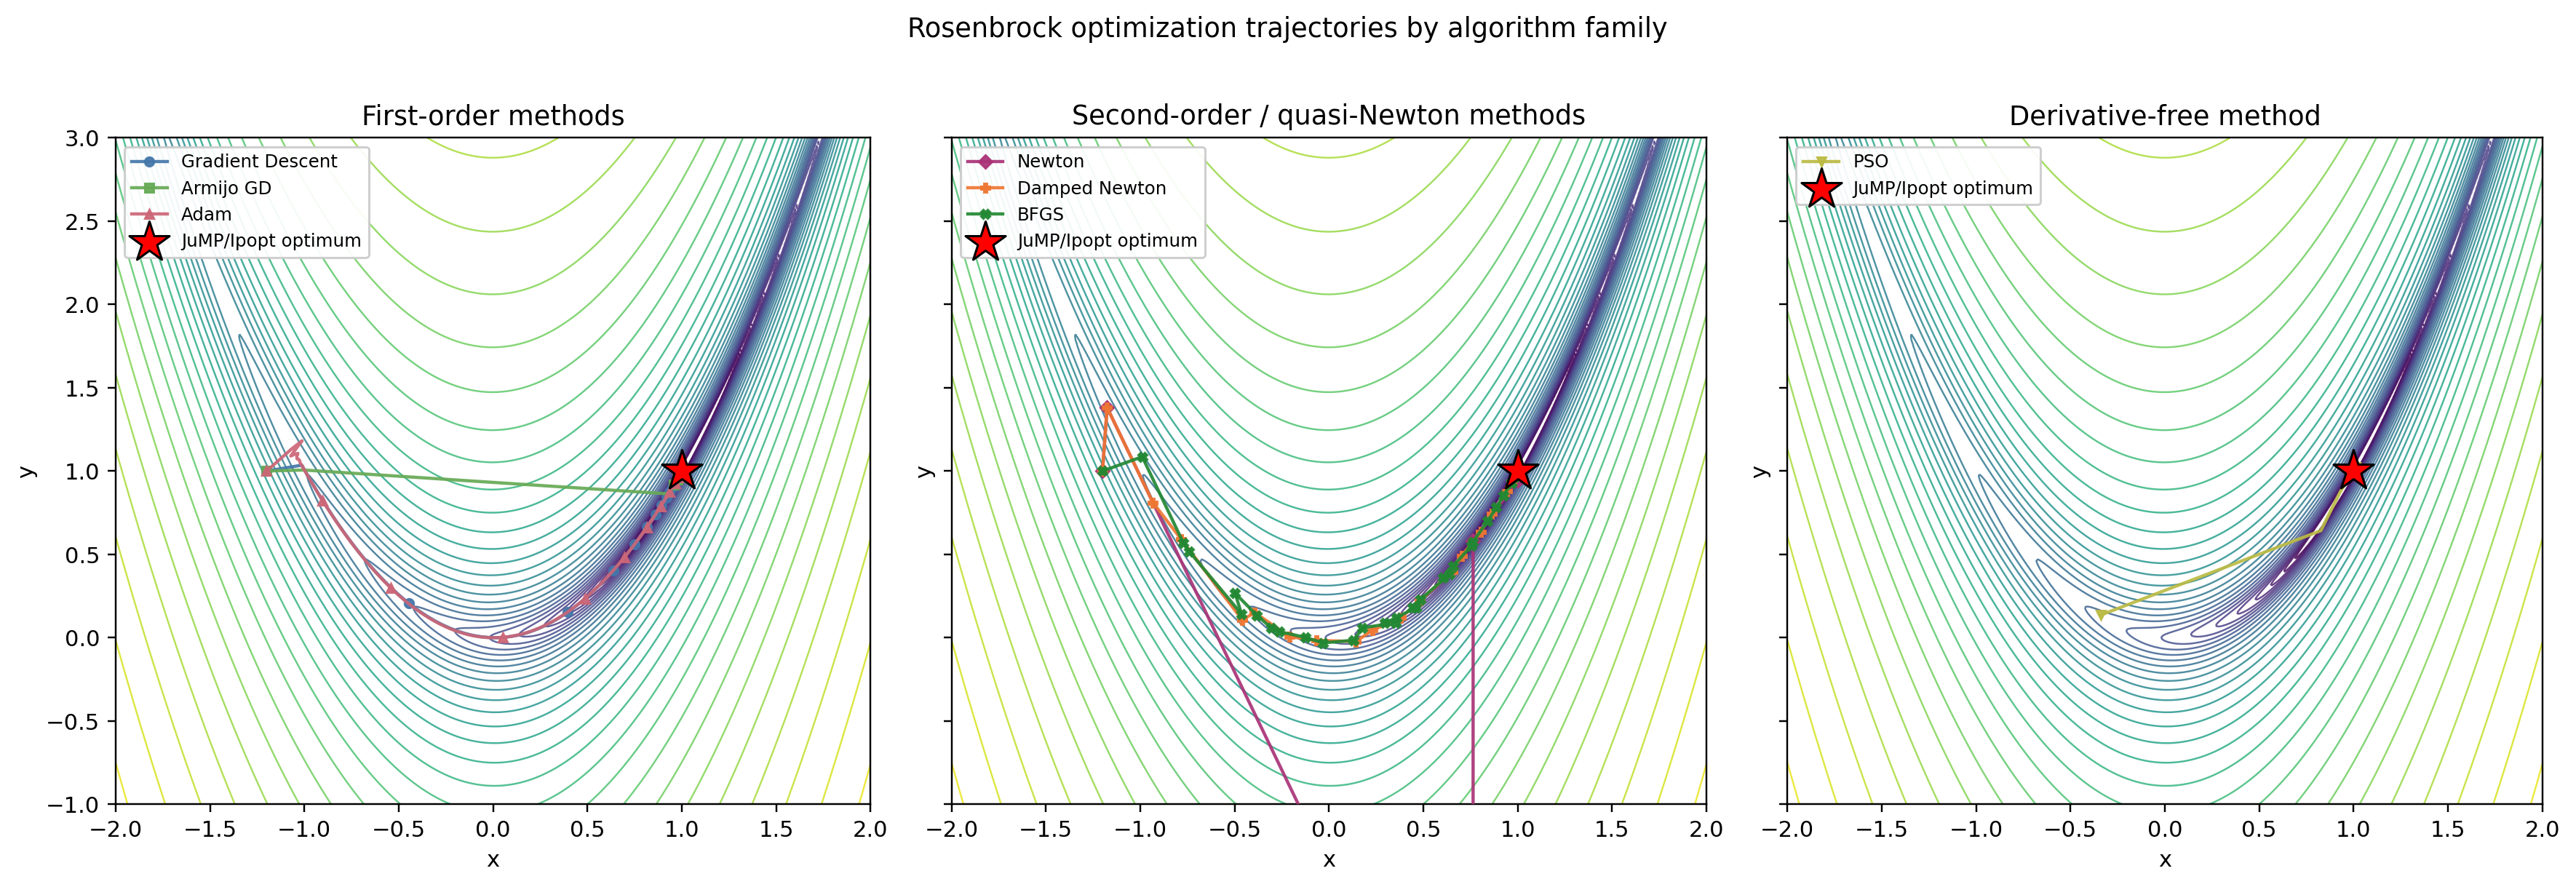
\includegraphics[width=0.98\textwidth,height=0.58\textheight,keepaspectratio]{rosenbrock_contours_trajectories.png}
\caption{Rosenbrock 函数等高线与各类算法迭代轨迹}
\end{figure}

图 1 将算法按一阶、二阶/拟二阶、无导数三类分开展示。背景采用白底彩色等高线而非填充色块，既保留函数值变化的层次，也避免背景遮挡轨迹线。可以看到，一阶方法沿 Rosenbrock 谷地缓慢推进，Adam 的轨迹较平滑；Newton 类方法会出现更大的曲率校正步，但很快进入最优点附近；PSO 展示的是群体最优点变化，不应按连续梯度轨迹理解。红色五角星表示 JuMP/Ipopt 基准点，并被绘制在最上层。

\begin{figure}[H]
\centering
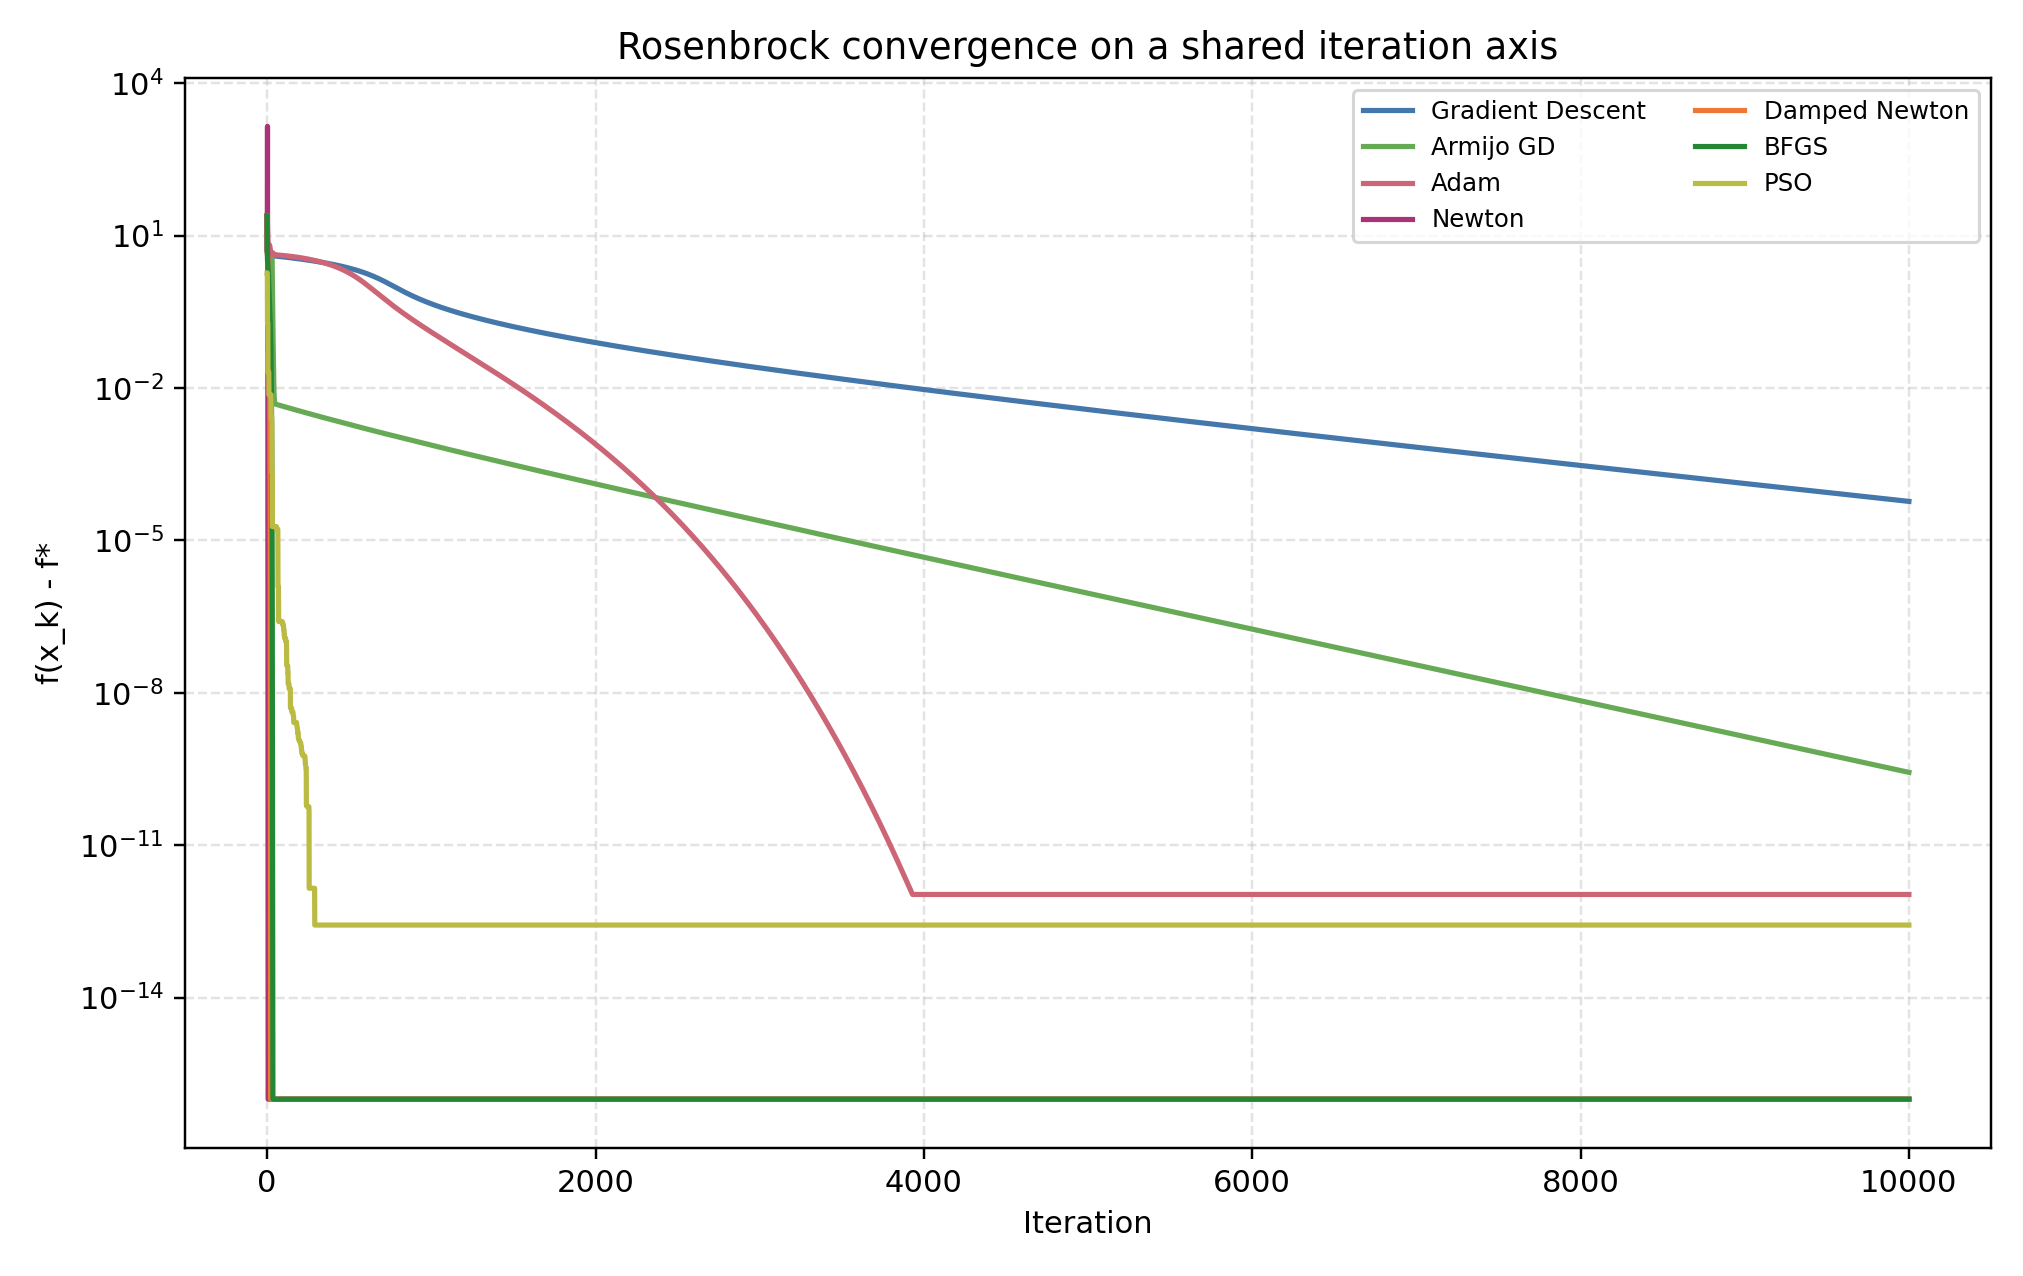
\includegraphics[width=0.94\textwidth,height=0.50\textheight,keepaspectratio]{rosenbrock_convergence.png}
\caption{Rosenbrock 函数收敛曲线}
\end{figure}

图 2 使用统一横轴绘制 $f(x_k)-f^*$。对于已经提前达到收敛阈值的方法，曲线在后续横轴上保持最终值，这样可以在同一迭代尺度下比较所有算法。图中可以看到，一阶方法需要大量迭代逐渐降低目标函数；Newton、阻尼 Newton 和 BFGS 在早期迅速下降并进入平台区。

\begin{figure}[H]
\centering
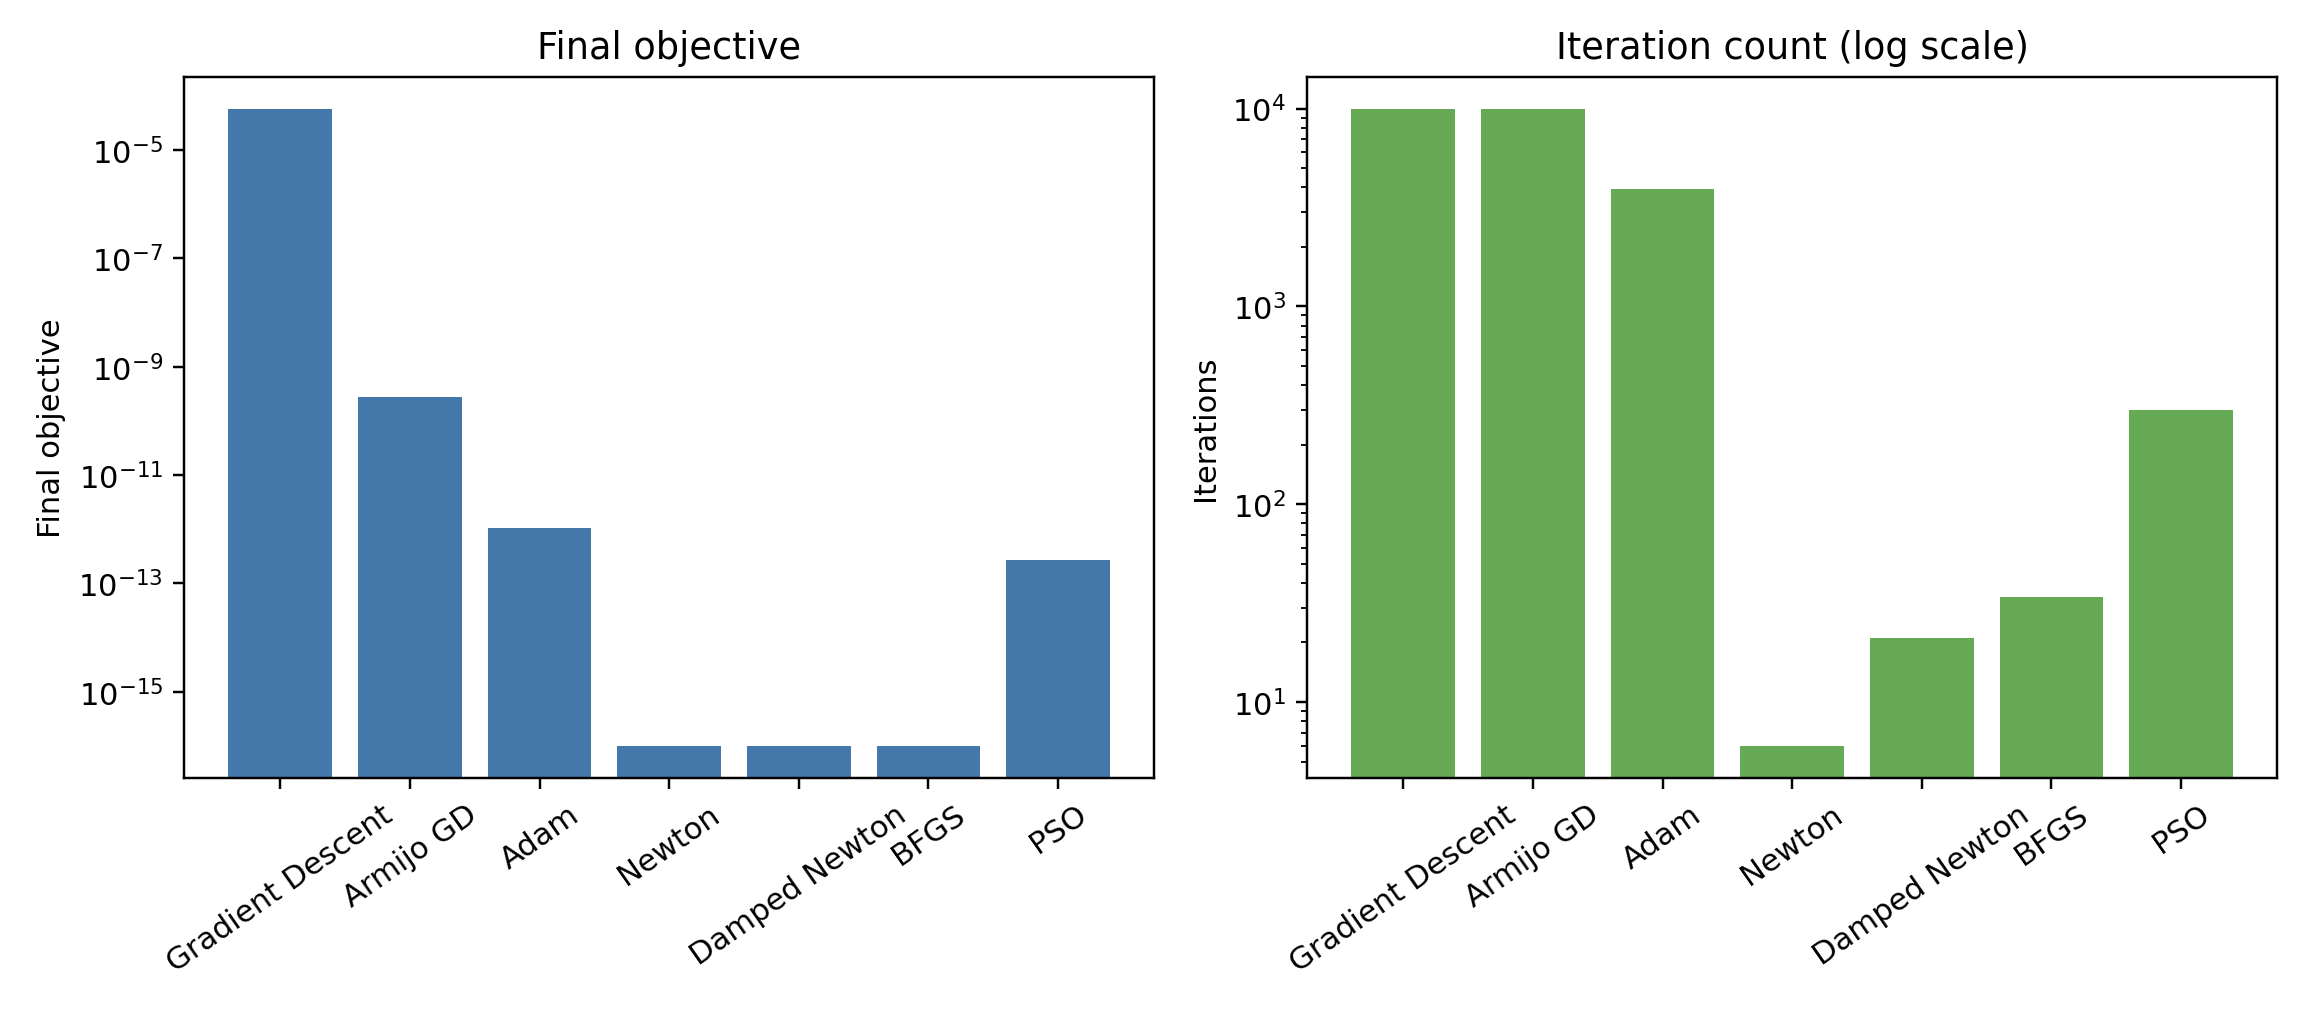
\includegraphics[width=0.94\textwidth,height=0.50\textheight,keepaspectratio]{rosenbrock_algorithm_comparison.png}
\caption{Rosenbrock 算法最终目标值与迭代次数对比}
\end{figure}

图 3 比较最终目标函数和迭代次数。由于不同方法迭代次数差异很大，右图使用对数坐标轴，避免 Newton、阻尼 Newton 和 BFGS 的柱子在普通坐标下几乎不可见。该图强调了两个事实：从最终精度看，多数算法都能接近最优；从迭代效率看，二阶和拟二阶方法明显占优。

\subsection{ADMM-Lasso 结果分析}

\begin{table}[H]
\centering
\scriptsize
\resizebox{\textwidth}{!}{%
\begin{tabular}{lrrrrrr}
\toprule
方法 & 迭代数 & 最终目标值 & primal residual & dual residual & 稀疏率 & 相对误差 \\
\midrule
ADMM-Lasso & 300 & $8.7276\times10^{-1}$ & $1.3617\times10^{-16}$ & $0.0000\times10^{0}$ & 86.00\% & $5.3862\times10^{-2}$ \\
\bottomrule
\end{tabular}
}
\caption{ADMM-Lasso 稀疏回归结果}
\end{table}

\begin{figure}[H]
\centering
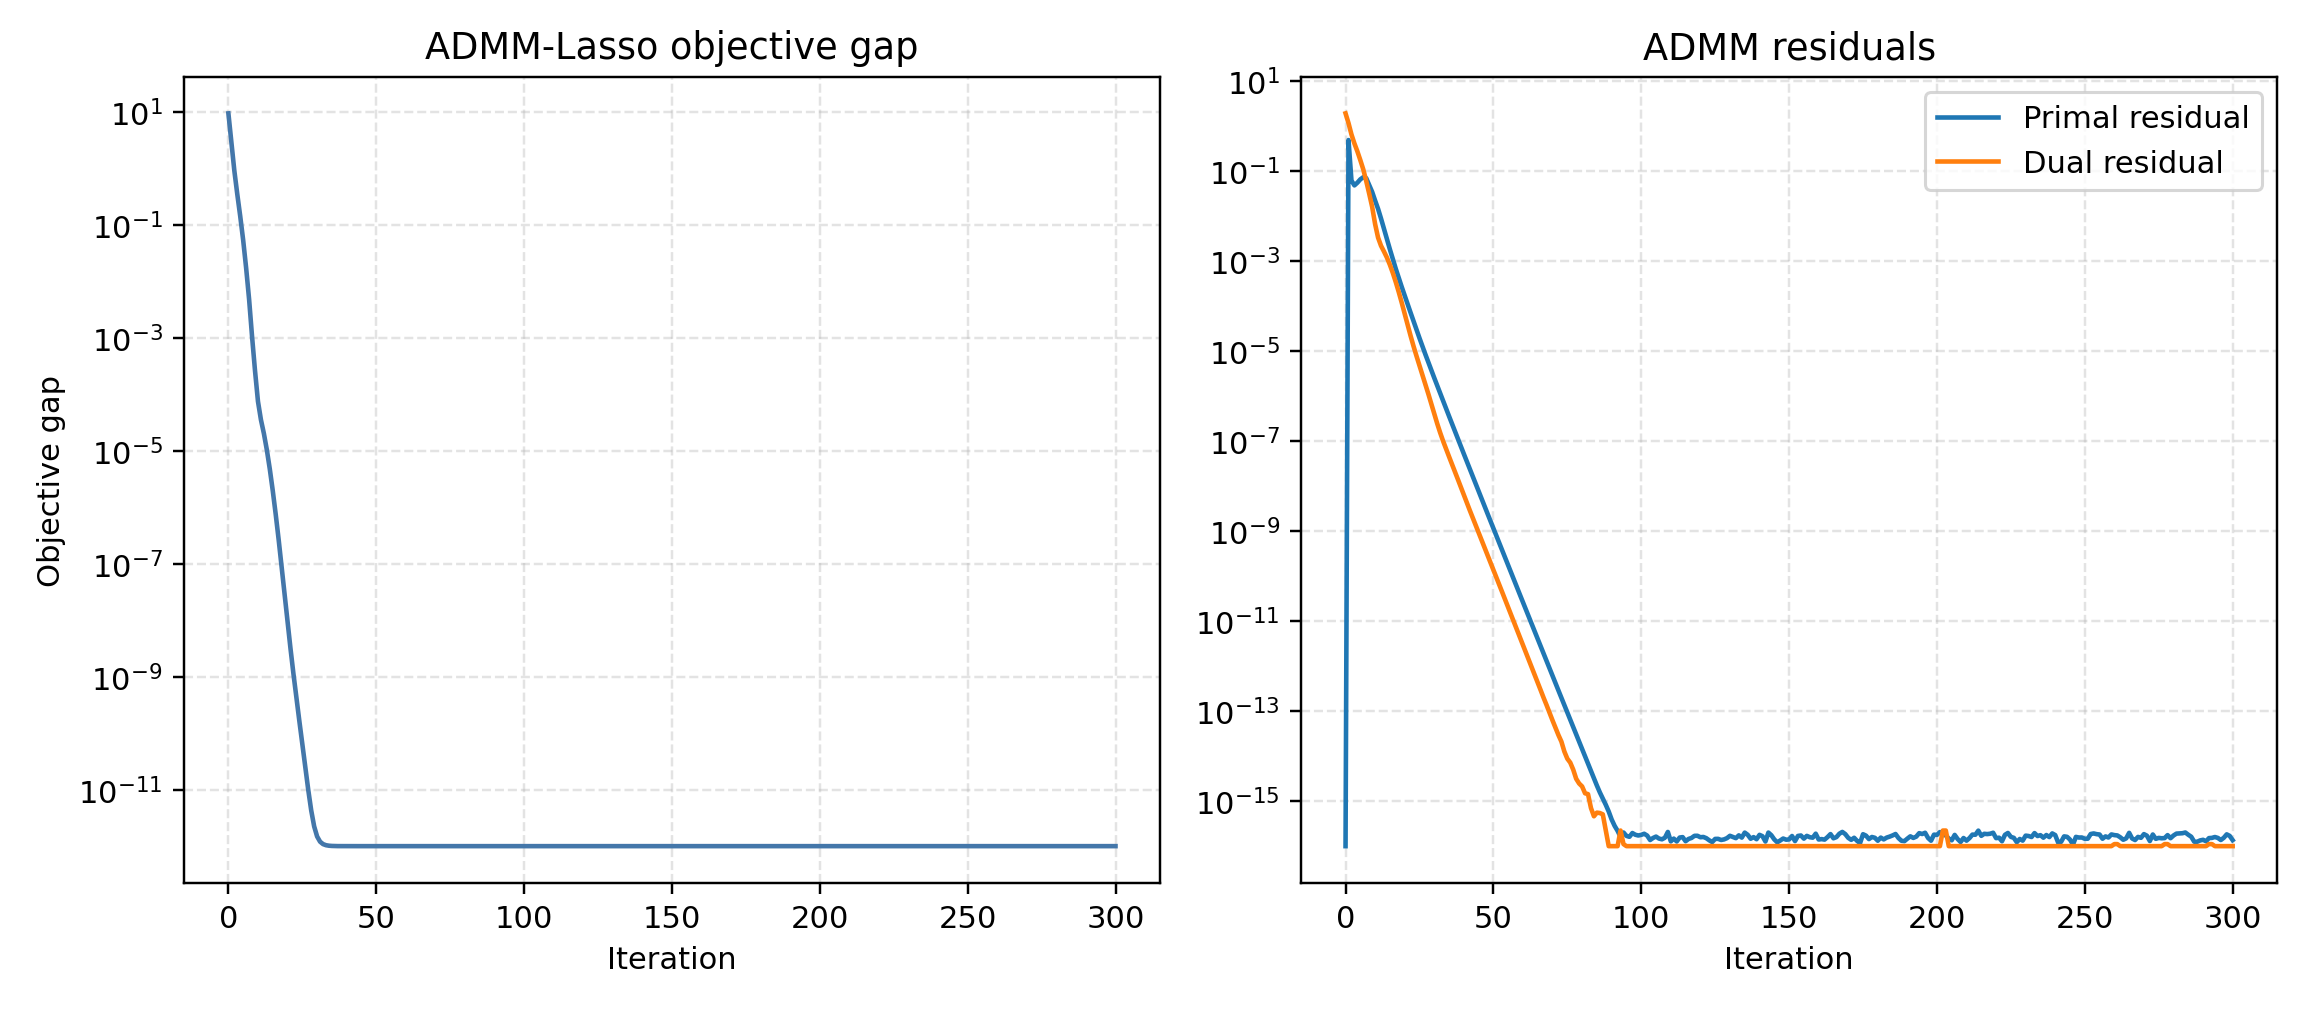
\includegraphics[width=0.94\textwidth,height=0.50\textheight,keepaspectratio]{admm_lasso_objective_residuals.png}
\caption{ADMM-Lasso 目标函数 gap 和残差}
\end{figure}

图 4 左侧绘制目标函数相对最终最小值的 gap，并使用对数坐标轴。这样可以观察快速下降阶段和后期平台阶段。右侧绘制 primal residual 和 dual residual，二者都使用对数坐标轴。残差前期下降较快，后期接近机器精度后变平，这是数值算法中常见的稳定现象。

\begin{figure}[H]
\centering
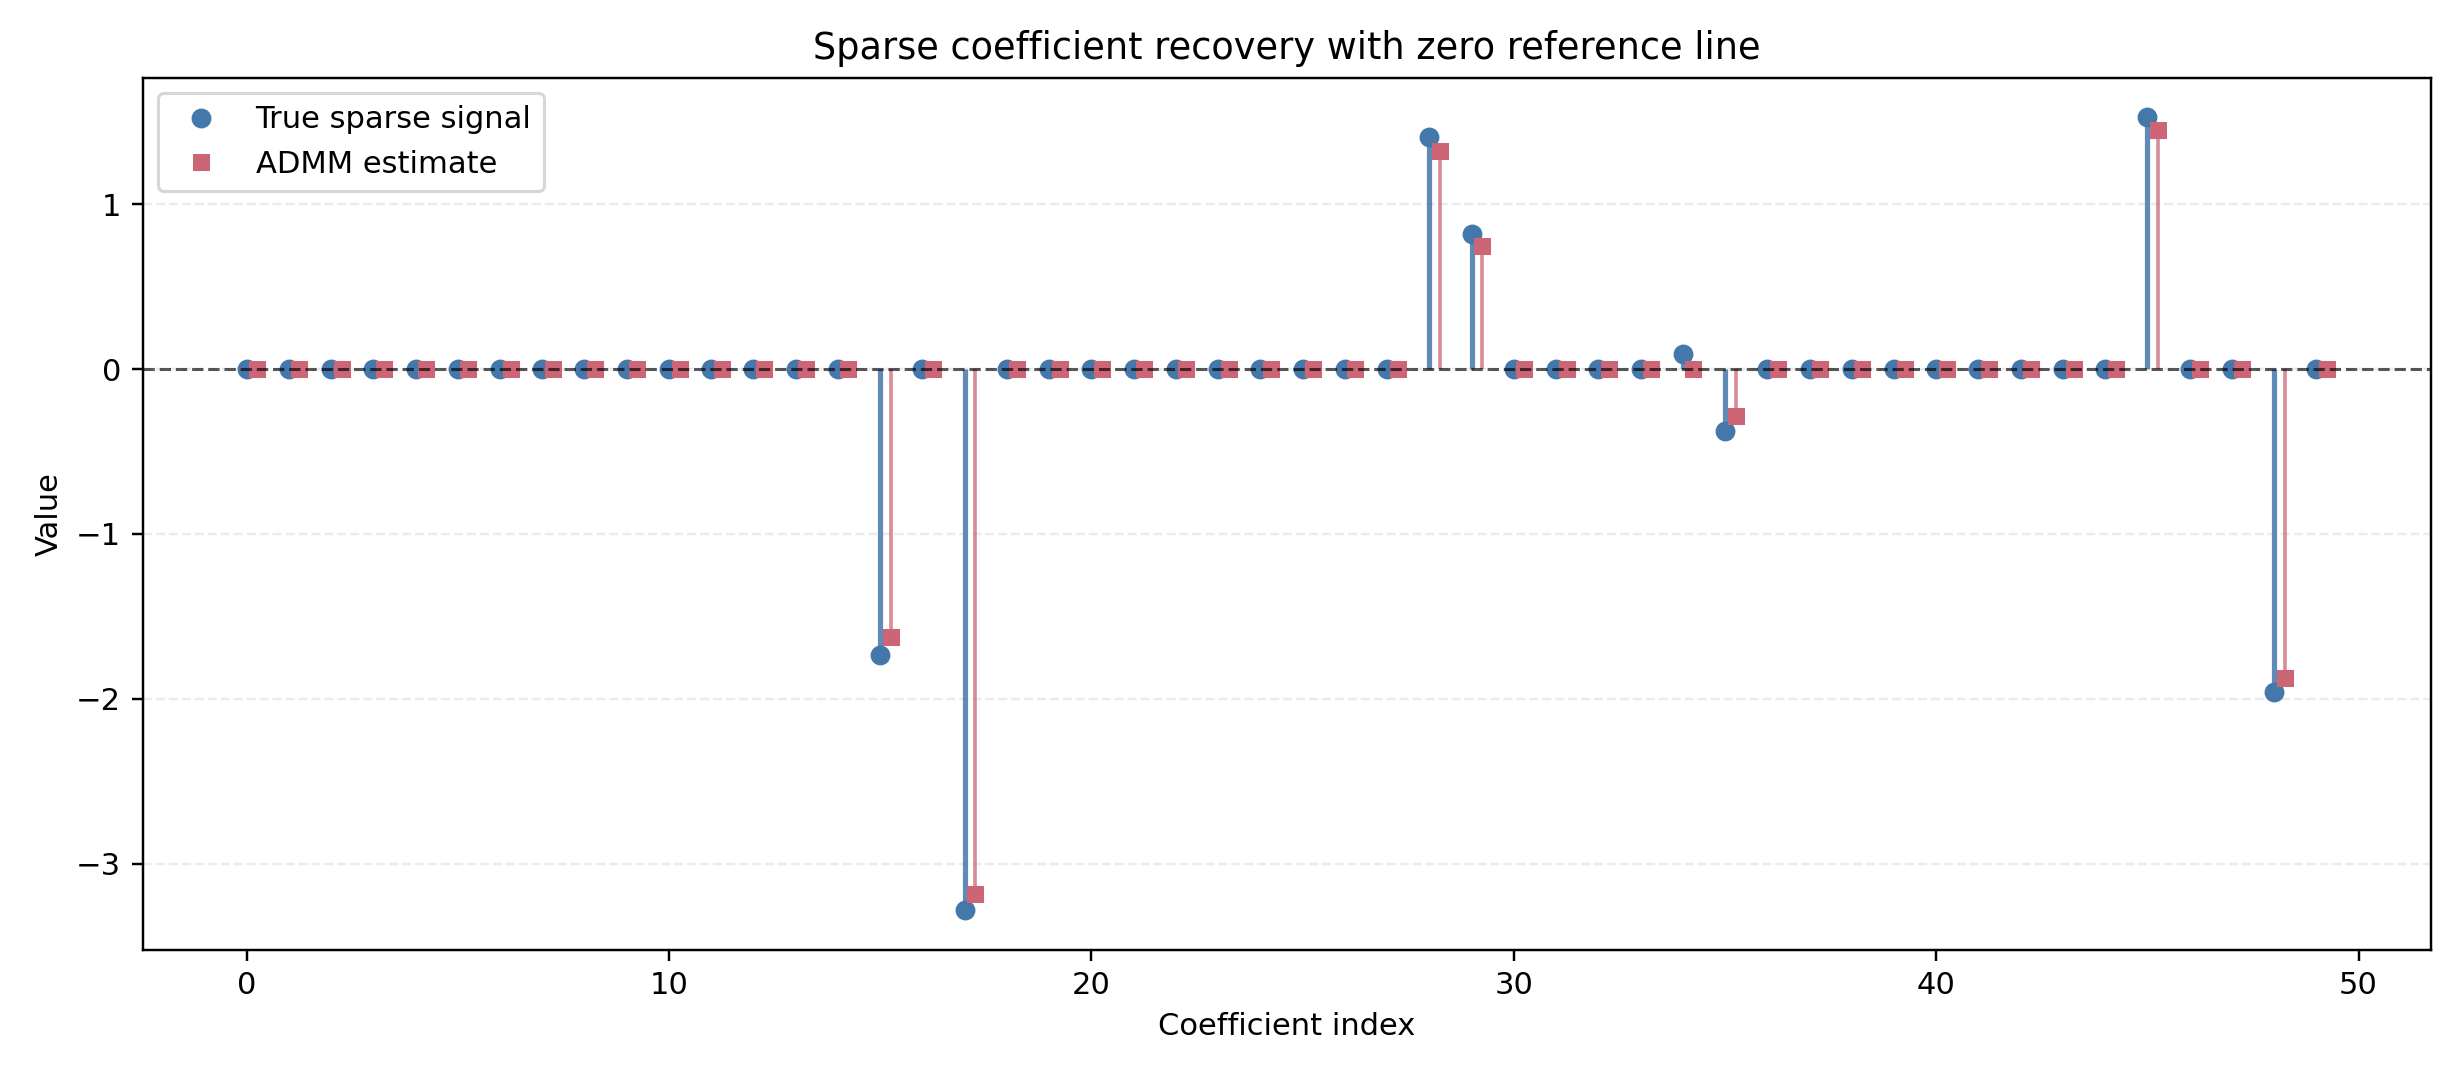
\includegraphics[width=0.94\textwidth,height=0.50\textheight,keepaspectratio]{admm_lasso_solution_recovery.png}
\caption{ADMM-Lasso 稀疏解恢复}
\end{figure}

图 5 对比真实稀疏系数和 ADMM 恢复系数，并加入 $y=0$ 的横向虚线。由于真实信号本身大部分坐标为零，图中大量位置接近零是 Lasso 稀疏模型的预期结果。零线可以帮助观察哪些系数被压到零，哪些位置保留了显著非零值。

\section{总结}

本实验完成了一个结构清晰、可复现的优化算法测试平台，并围绕 Rosenbrock 函数和 Lasso 问题验证了多类优化方法。实验得到以下结论：

\begin{enumerate}
\item JuMP/Ipopt 可以作为可靠的基准求解器，用来校验手写算法在测试函数上的结果。
\item 固定步长 GD 稳定但收敛慢；Armijo 线搜索能显著改善固定步长问题，但在 Rosenbrock 谷地中仍需要大量迭代。
\item Adam 的自适应缩放提升了一阶方法的实用性，在本实验中能达到严格梯度收敛阈值。
\item Newton、阻尼 Newton 和 BFGS 利用曲率信息后迭代效率明显更高，尤其适合低维且目标函数可微的测试问题。
\item PSO 不需要梯度，在低维连续优化中也能找到较高质量近似解，但其轨迹解释应区别于梯度方法。
\item ADMM 通过变量分裂把光滑损失和非光滑 L1 正则分开处理，软阈值步骤能够产生严格稀疏解。
\end{enumerate}

从课程实验角度看，本实验覆盖了 JuMP、一阶算法、二阶算法、无导数算法、ADMM、测试函数、收敛曲线、迭代轨迹和结果对比等要求。后续可以继续在该平台中扩展共轭梯度法、Krylov 子空间法、三次正则化 Newton 法，以及更多带约束优化问题。

\newpage
\section{参考文献}

\begin{enumerate}
\item Stephen Boyd and Lieven Vandenberghe. \textit{Convex Optimization}. Cambridge University Press, 2004.
\item Stephen Boyd, Neal Parikh, Eric Chu, Borja Peleato, and Jonathan Eckstein. Distributed Optimization and Statistical Learning via the Alternating Direction Method of Multipliers. \textit{Foundations and Trends in Machine Learning}, 2011.
\item Jorge Nocedal and Stephen Wright. \textit{Numerical Optimization}. Springer, 2006.
\item Diederik P. Kingma and Jimmy Ba. Adam: A Method for Stochastic Optimization. ICLR, 2015.
\item James Kennedy and Russell Eberhart. Particle Swarm Optimization. IEEE International Conference on Neural Networks, 1995.
\item Miles Lubin, Oscar Dowson, Joaquim Dias Garcia, Joey Huchette, Benoit Legat, and Juan Pablo Vielma. JuMP 1.0: Recent improvements to a modeling language for mathematical optimization. \textit{Mathematical Programming Computation}, 2023.
\end{enumerate}

\newpage
\section{附录：代码与结果目录说明}

\begingroup
\scriptsize
\begin{longtable}{p{0.66\textwidth}p{0.24\textwidth}}
\toprule
路径 & 说明 \\
\midrule
\texttt{tools/Experiment1\_Optimization\_Platform/run\_all.py} & 一键运行全部实验 \\
\texttt{tools/Experiment1\_Optimization\_Platform/src/first\_order.py} & 固定步长 GD、Armijo GD、Adam \\
\texttt{tools/Experiment1\_Optimization\_Platform/src/second\_order.py} & Newton、阻尼 Newton、BFGS \\
\texttt{tools/Experiment1\_Optimization\_Platform/src/derivative\_free.py} & PSO \\
\texttt{tools/Experiment1\_Optimization\_Platform/src/admm\_lasso.py} & ADMM-Lasso \\
\texttt{tools/Experiment1\_Optimization\_Platform/src/jump\_baseline.py} & JuMP 基准调用与备用校验逻辑 \\
\texttt{tools/Experiment1\_Optimization\_Platform/julia/jump\_rosenbrock.jl} & JuMP/Ipopt Rosenbrock 求解脚本 \\
\texttt{report\_assets/Experiment1\_Optimization\_Platform/raw/} & 原始 JSON 结果 \\
\texttt{report\_assets/Experiment1\_Optimization\_Platform/tables/} & CSV 汇总表 \\
\texttt{report\_assets/Experiment1\_Optimization\_Platform/figures/} & 报告图片 \\
\texttt{Latex/Experiment1\_Optimization\_Platform/} & LaTeX 源文件与 PDF \\
\bottomrule
\end{longtable}
\endgroup

\newpage
\section{附录：核心算法代码摘录}

本附录只列出报告讲解中最关键的实现片段。完整代码位于实验一工具目录；这里保留目标函数、线搜索、主要更新公式和 JuMP 建模代码，便于对照正文解释算法流程。

\subsection{Rosenbrock 函数、梯度、Hessian 与 Armijo 线搜索}

\begin{lstlisting}[language=Python]
def rosenbrock(x):
    return float((1.0 - x[0]) ** 2 + 100.0 * (x[1] - x[0] ** 2) ** 2)

def rosenbrock_grad(x):
    return np.array([
        -2.0 * (1.0 - x[0]) - 400.0 * x[0] * (x[1] - x[0] ** 2),
        200.0 * (x[1] - x[0] ** 2),
    ])

def rosenbrock_hessian(x):
    return np.array([
        [2.0 - 400.0 * x[1] + 1200.0 * x[0] ** 2, -400.0 * x[0]],
        [-400.0 * x[0], 200.0],
    ])

def armijo_backtracking(f, grad, x, direction, alpha0=1.0, c1=1e-4, beta=0.5):
    alpha = alpha0
    fx = f(x)
    slope = float(np.dot(grad(x), direction))
    while alpha > 1e-12:
        if f(x + alpha * direction) <= fx + c1 * alpha * slope:
            return alpha
        alpha *= beta
    return 1e-12
\end{lstlisting}

\subsection{一阶算法：梯度下降与 Adam}

\begin{lstlisting}[language=Python]
def gradient_descent(f, grad, x0, lr=1e-3, max_iter=10000, tol=1e-6):
    x = np.asarray(x0, dtype=float).copy()
    history = []
    for _ in range(max_iter):
        g = grad(x)
        history.append({"x": x.copy(), "f": f(x), "grad_norm": np.linalg.norm(g)})
        if np.linalg.norm(g) < tol:
            break
        x = x - lr * g
    return x, history

def adam(f, grad, x0, lr=0.02, beta1=0.9, beta2=0.999, eps=1e-8):
    x = np.asarray(x0, dtype=float).copy()
    m = np.zeros_like(x)
    v = np.zeros_like(x)
    history = []
    for k in range(1, 10001):
        g = grad(x)
        history.append({"x": x.copy(), "f": f(x), "grad_norm": np.linalg.norm(g)})
        if np.linalg.norm(g) < 1e-6:
            break
        m = beta1 * m + (1.0 - beta1) * g
        v = beta2 * v + (1.0 - beta2) * (g * g)
        m_hat = m / (1.0 - beta1**k)
        v_hat = v / (1.0 - beta2**k)
        x = x - lr * m_hat / (np.sqrt(v_hat) + eps)
    return x, history
\end{lstlisting}

\subsection{二阶与拟二阶算法：Newton、阻尼 Newton 和 BFGS}

\begin{lstlisting}[language=Python]
def newton_direction(hess_matrix, grad_vector):
    try:
        return -np.linalg.solve(hess_matrix, grad_vector)
    except np.linalg.LinAlgError:
        return -np.linalg.pinv(hess_matrix) @ grad_vector

def damped_newton_step(f, grad, hess, x):
    g = grad(x)
    direction = newton_direction(hess(x), g)
    if float(np.dot(g, direction)) >= 0.0:
        direction = -g
    alpha = armijo_backtracking(f, grad, x, direction)
    return x + alpha * direction

def bfgs_update(h_inv, s, y):
    ys = float(np.dot(y, s))
    if ys <= 1e-12:
        return h_inv
    rho = 1.0 / ys
    eye = np.eye(len(s))
    return (eye - rho * np.outer(s, y)) @ h_inv @ (
        eye - rho * np.outer(y, s)
    ) + rho * np.outer(s, s)
\end{lstlisting}

\subsection{无导数算法：粒子群优化 PSO}

\begin{lstlisting}[language=Python]
positions = rng.uniform(lower, upper, size=(particles, dim))
velocities = rng.uniform(-0.1 * span, 0.1 * span, size=positions.shape)
personal_best = positions.copy()
personal_values = np.array([f(p) for p in positions])
global_best = personal_best[np.argmin(personal_values)].copy()

for _ in range(iterations):
    r1 = rng.random(size=positions.shape)
    r2 = rng.random(size=positions.shape)
    velocities = (
        w * velocities
        + c1 * r1 * (personal_best - positions)
        + c2 * r2 * (global_best - positions)
    )
    positions = np.clip(positions + velocities, lower, upper)
    values = np.array([f(p) for p in positions])
    improved = values < personal_values
    personal_best[improved] = positions[improved]
    personal_values[improved] = values[improved]
    global_best = personal_best[np.argmin(personal_values)].copy()
\end{lstlisting}

\subsection{ADMM-Lasso：软阈值和三步迭代}

\begin{lstlisting}[language=Python]
def soft_threshold(v, kappa):
    return np.sign(v) * np.maximum(np.abs(v) - kappa, 0.0)

x = np.zeros(n)
z = np.zeros(n)
u = np.zeros(n)
lhs = A.T @ A + rho * np.eye(n)
atb = A.T @ b

for _ in range(iterations):
    x = np.linalg.solve(lhs, atb + rho * (z - u))
    z_old = z.copy()
    z = soft_threshold(x + u, lam / rho)
    u = u + x - z
    primal_residual = np.linalg.norm(x - z)
    dual_residual = rho * np.linalg.norm(z - z_old)
\end{lstlisting}

\subsection{Julia/JuMP 基准求解器}

\begin{lstlisting}
using JuMP
using Ipopt
using JSON

model = Model(Ipopt.Optimizer)
set_silent(model)
@variable(model, x)
@variable(model, y)
@NLobjective(model, Min, (1 - x)^2 + 100 * (y - x^2)^2)
optimize!(model)

result = Dict(
    "x" => value(x),
    "y" => value(y),
    "objective" => objective_value(model),
    "termination_status" => string(termination_status(model)),
)
\end{lstlisting}

\end{document}
